\chapter{Rotårsaksidentifisering}
Arbeidet i denne fasen går ut på å identifisere rotårsaken. I foregående fasen ble en rekke mulige årsaker identifisert og analysert, men nå er det tid for å finne den faktiske rotårsaken. Det er mange forskjellige verktøy som kan brukes i denne fasen, men vi har brukt et 5 whys og feiltreanalyse for vårt utgangspunkt. 

\section{5 whys}
5 Whys er et verktøy som prøver å gjøre et dypdykk i årsakene for å finne rotårsaken. Måten dette gjøres på er å hele tiden spørre ``Why?'', altså hvorfor på norsk, hver gang en ny årsak dukker opp. Det brukes ofte for å sjekke om de identifiserte årsakene er symptomer, lav-nivå årsaker eller rotårsaker. 

\subsection{Ønsket utbytte}
Ved å bruke 5 Whys prøver vi å finne ut hva som er rotårsaken til problemet.

\subsection{Gjennomføring}
Med dette verktøyet tar vi utgangspunkt i casebeskrivelsen; nemlig rotårsaken til kryptoutvinning på NTNU. Ut fra dette brukte vi funnene fra analysen for å komme på årsaker, samt prøvde å idémyldre et par nye. For hver av disse årsakene ble det spurt: ``Hvorfor er dette en årsak av det originale problemet?''. For hvert svar spør vi hvorfor igjen og igjen helt til vi finner rotårsaken. Det ble tatt utgangspunkt i fem iterasjoner, men det er mulighet for flere eller færre avhengig av om spørsmålet kan besvares på en fornuftig måte. 

\subsection{Resultater}
Det ble fremhevet fem årsaker som skulle analyseres. Fire av disse kom fra fiskebeindiagrammet over, og en fra idémyldring. Tabellene under viser resultatene fra gjennomføringen. 

\begin{table} [H]
    \centering
    \begin{tabular}{ | m{5em} | m{30em} | }
        \hline
            \cellcolor{yellow} Årsak: & \cellcolor{yellow} Ansatte og studenter utvinner krypto med universitetet sine ressurser                \\
        \hline
            Why? & Lønnsomhet                                    \\
        \hline
            Why? & Har ingen utgifter                                            \\
        \hline
            Why? & Bruker strøm og infrastrukturen til skolen                \\
        \hline
            Why? & Det er en gråsone i regelverket           \\
        \hline
            Why? & Ikke spesifisert godt nok i IT-reglementet   \\
        \hline
    \end{tabular}
    \caption[5 Whys: Ansatte og studenter utvinner krypto med skolens]{5 Whys på ansatte og studenter utvinner krypto med skolens}
    \label{5Whys-interne}
\end{table}
Det å utvinne krypto på universitetet sine ressurser er alt fra å kjøre en kryptominer på en PC til å sette opp en mining rig. I 5 Whys over kom vi frem til at lønnsomhet er primærgrunnen til at de driver med kryptoutvinning, men årsaken til at ansatte og studenter utvinner på universitet er at det ikke er spesifisert godt nok i IT-reglementet.   


\begin{table} [H]
    \centering
    \begin{tabular}{ | m{5em} | m{30em} | }
        \hline
            \cellcolor{yellow} Årsak: & \cellcolor{yellow} Eksterne trusselaktører utvinner krypto med skolens ressurser              \\
        \hline
            Why? & Lønnsomhet                                   \\
        \hline
            Why? & Enkelt å spre minere                                           \\
        \hline
            Why? & Folk går inn på waterholes og trykker på phishingmail               \\
        \hline
            Why? & Brukeren var ikke oppmerksom nok på e-mailen eller siden de gikk på           \\
        \hline
            Why? & Brukere har ikke fått nok opplæring i hvordan dette unngås    \\
        \hline
    \end{tabular}
    \caption[5 Whys: Eksterne trusselaktører utvinner krypto med skolens ressurser]{5 Whys Eksterne trusselaktører utvinner krypto med skolens ressurser}
    \label{5Whys-eksterne}
\end{table}

Årsaken til at eksterne trusselaktører utvinner krypto med skolen sine ressurser er fordi det er en lønnsom affære som er koster lite å distribuere og som det er liten sannsynlighet for å bli tatt for. Med eksterne trusselaktører mener vi folk som utvinner på andre sine datamaskiner gjennom å få skadevare installert på disse.

\begin{table} [H]
    \centering
    \begin{tabular}{ | m{5em} | m{30em} | }
        \hline
            \cellcolor{yellow} Årsak: & \cellcolor{yellow} Utvinnere som implementert inn i nettsider              \\
        \hline
            Why? & God fortjeneste                                   \\
        \hline
            Why? & Fordi de når en stor menge folk som utvinner krypto for dem                                           \\
        \hline
            Why? & Mange har ikke en annonseblokkering som også stopper utvinnere på nett               \\
        \hline
            Why? & På grunn av lite eller ingen opplæring til denne typen programvare           \\
        \hline
            Why? & Ikke prioritert    \\
        \hline
            Why? & Fordi det ikke er nok folk/ressurser    \\
        \hline
    \end{tabular}
    \caption[5 Whys: Minere som er implementert inn i nettsider]{5 Whys på ansatte og studenter utvinner krypto med skolens}
    \label{5Whys-minere}
\end{table}
Årsaken til at nettsider som har muligheten til å utvinne kryptovaluta er et problem er fordi, de starter å bli utbredt og de spør ofte ikke om godkjenning for utvinning på PCene til folk.

\subsection{Konklusjon av verktøy}
Verktøyet var svært nyttig for å gå dypt inn i årsakene. Et problem består ofte av flere nivåer av årsaker, og det tar 5 Whys hensyn til. I forhold til informasjonssikkerhet burde man passe på å ikke alltid ende opp med en årsak som er relatert til IT-reglement, da problemet ofte også kan være av teknisk art. Dette var en mulig fallgruve for oss, men det er usikkert om det bare gjelder dette caset. Et annet problem med verktøyet er at det kan bli for ensporet på en spesifikk tankegang. Det kan derfor anbefales i noen tilfeller å undersøke samme årsaken flere ganger dersom det er grunn til å tro at det finnes flere relevante 
årsaker ved ett av spørsmålene, som fører til en annen rotårsak.

\section{Feiltreanalyse}
Feiltreanalyse tar alle mulige årsaker i et diagram og identifiserer mulige linker. Analysen bygger på hva som ble gjort i 5 Whys. 

\subsection{Ønsket utbytte}
Ved bruk av dette verktøyet ønsker vi å få en oversikt over koblinger mellom de forskjellige årsakene. Vi ønsker også å få sortert ut de årsakene som NTNU ikke har mulighet til å gjøre.

\subsection{Gjennomføring}
Med dette verktøy tar vi utgangspunktet i resultatet fra 5 Whys til å finne rotårsakene. Her går vi steg for steg nedover og ser på hva som er årsaken til at enhver uønsket hendelse inntreffer.

\subsection{Resultater}
Vi har kommet fram til fire hovedgrunner til at kryptoutvinning på NTNU forekommer. Rotårsaken er sammensatt av disse årsakene definert i figur \ref{fig:feil_tre_analyse}. I dette caset er problemet delt inn i to deler; de interne og de eksterne. Det er to forskjellige typer årsaker, der interne går mer på regelverk og eksterne er mer teknisk.          

I figur \ref{fig:feil_tre_analyse} representerer trekanter ``eller'', halvsirkelen representer ``og''. De røde boksene er de årsakene vi ikke kan gjøre noe med, de grønne kan det gjøres noe med.
 \begin{figure}[H]
    \centering
    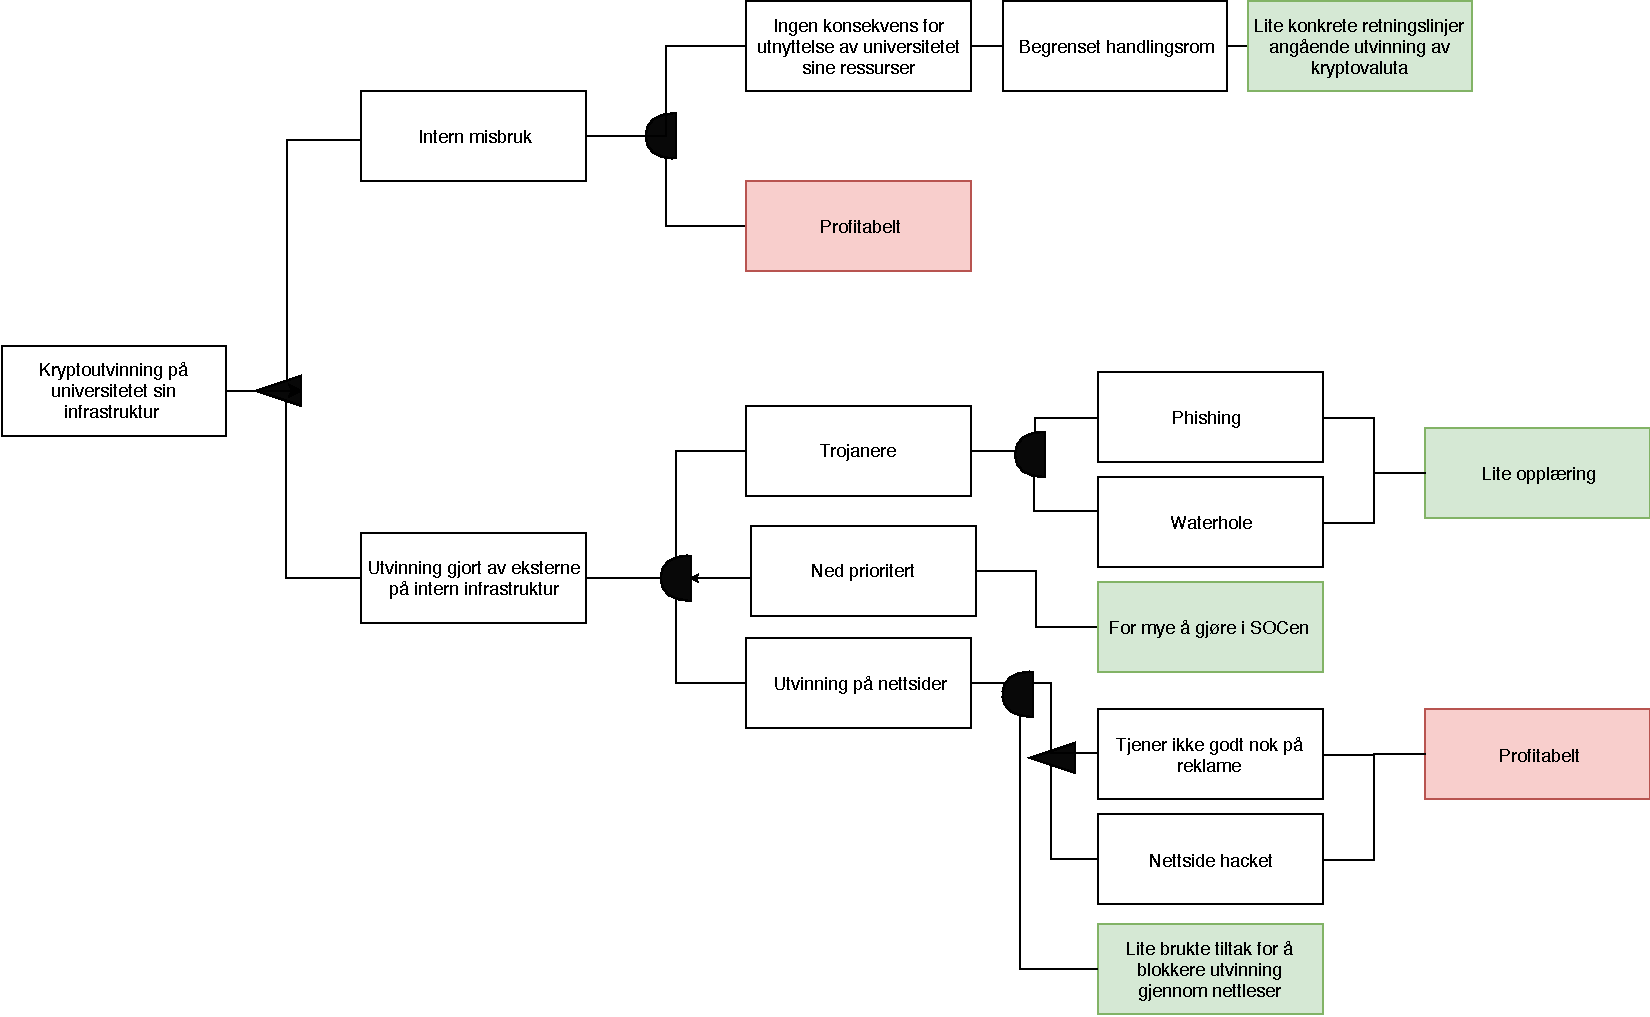
\includegraphics[scale=0.45]{case_3/bilder/feil_tre_analyse.pdf}
    \caption[Feiltreanalyse]{Feiltreanalyse}
    \label{fig:feil_tre_analyse}
\end{figure}

\subsection{Konklusjon av verktøy}
Verktøyet funger godt til å se hvordan de forskjellige årsakene er koblet sammen og hva som er hovedårsakene. Der man ser hvordan interne og eksterne er koblet sammen og hvordan de er forskjellige. 